%% -*- eval: (flyspell-mode 1); -*-

\chapter{Bibliothèque de stencils basée sur \textsf{SYCL}}

Au cours du stage a été développé un DSEL de stencils sous la forme d'une bibliothèque \textsf{C++}. Ce DSEL essaie de reprendre les objectifs explicités dans le chapitre précédent. Toutefois il s'agit plutôt d'une preuve de faisabilité ce pour quoi tous les objectifs n'ont pas été implémentés (mais leur intégration a été prévue). Ce chapitre se concentre sur la présentation de ce DSEL en ce qui concerne son utilisation, quelques détails d'implantation, ainsi que le travail restant.

\section{Présentation générale}

Le DSEL implémenté s'appuie sur deux classes pour les coefficients (constants ou variables), plusieurs classes pour la description d'une opération (tableaux d'entrée et de sortie, fonctions d'accès aux éléments ou aux coefficients telles que décrites dans la section \ref{sec:obj_sem}) et une unique classe pour lancer les calculs. L'implantation ne concerne que des stencils en deux dimensions. L'écriture d'un problème à base de stencils dans le DSEL se fait en cinq étapes :

\begin{enumerate}
\item initialiser les coefficients ;
\item les assembler pour former un stencil au sein d'un objet \emph{stencil};
\item regrouper les informations nécessaires au calcul (stencil, tableaux et fonctions) au sein d'un objet \emph{operation};
\item déclarer une queue de calcul dans le formalisme \textsf{SYCL} ;
\item appeler la méthode de lancement des calcul sur l'objet \emph{operation}.
\end{enumerate}

Avant de présenter plus en détail l'interface pour la création des stencils puis pour leur application, il convient d'introduire la bibliothèque de parallélisme \textsf{\href{https://github.com/amd/triSYCL}{triSYCL}} implantant l'interface \textsf{SYCL}. En effet certains objets que l'utilisateur doit fournir au DSEL sont définis par \textsf{SYCL}.

\subsection{Utilisation de \textsf{triSYCL}}

\textsf{triSYCL} est une bibliothèque écrite en \textsf{C++14} par Ronan Keryell pour le compte d'\textsf{AMD}. Il s'agit d'un prototype d'implantation de \textsf{SYCL} dont le but est avant tout de pouvoir vérifier la faisabilité d'une telle interface. Ses objectifs sont notamment de faciliter le lancement de calculs sur du matériel parallèle, pour cela elle calque de nombreuses possibilités sur \textsf{OpenCL} tout en les simplifiant. Parmi ces possibilités se retrouvent notamment :
\begin{itemize} 
\item la découverte (potentiellement) automatique du matériel disponible sur la machine ;
\item la gestion automatique des transferts de données avec ces matériels (la mémoire globale des cartes graphiques principalement) ;
\item le lancement de \emph{noyaux} de calcul sur le matériel désiré, avec configuration possible des tailles de \emph{warps}.
\end{itemize}

Celle-ci utilise notamment les \emph{lambda fonctions} et le mot-clé \textsf{auto}, introduits à partir de \textsf{C++11} et augmentés en \textsf{C++14}. Outre les éléments de langages, \textsf{triSYCL} s'appuie également sur la bibliothèque \textsf{Boost} par exemple pour la gestion des tableaux multidimensionnels, ainsi que sur \textsf{OpenMP} pour une parallélisation naïve des boucles uniquement sur CPU. L'implantation actuelle de \textsf{triSYCL} ne comprend pas toutes les fonctions de l'interface \textsf{SYCL}. Toutefois elle est suffisante pour les besoins du DSEL.

Les objets \textsf{SYCL} que l'utilisateur doit manipuler sont au nombre de trois seulement : les \emph{buffers} qui sont en fait les tableaux utilisés par les calculs (il s'agit de \emph{smart containers} évoqués dans la section \ref{sec:biblio}), les \emph{accesseurs} qui permettent de simplement lire ou modifier les buffers, et enfin les \emph{queues} qui sont les piles de lancement des tâches de calculs. Les cas d'utilisation de ces objets sont inclus dans les codes présentés avec l'interface du DSEL, et les objets sont alors toujours précédés de l'espace de noms \textsf{sycl}.

\subsection{Création des stencils}

Les coefficients peuvent être créés en version constante ou variable, avec les indices de décalage spécifiés dans le \emph{template} de la classe, ils seront donc statiques. La logique de construction n'est pas exactement la même pour les deux classes puisque la version constante nécessite de préciser le type du coefficient (entier, flottant, etc\ldots) qui n'est alors pas connu par le biais du tableau de coefficients. L'extrait de code \ref{lst:1} contient la façon de créer les deux types de coefficients.
\begin{listing}[H]
\caption{Création de coefficients, avec leur indice de décalage.}
\label{lst:1}
\begin{minted}[frame=single]{cpp}
/* la valeur du coefficient est affectée à la construction */
coef_fxd2D<-1, 1, double> c2(0.2);
/* les valeurs du coefficient nécessiteront une fonction tierce */
coef_var2D<0, 0> c1;
\end{minted}
\end{listing}

Une fois les coefficients initialisés, il est possible de les rassembler pour former le motif du stencil comme dans le code \ref{lst:2}. Il est d'ailleurs possible de combiner plusieurs stencils ensemble de la même manière. Toutefois il n'est possible d'agréger que des coefficients constants et du même type entre eux, ou bien que des coefficients variables entre eux. Il n'est pas possible de mélanger les deux possibilités.
\begin{listing}[H]
\caption{Agrégation des coefficients pour former un stencil à cinq points.}
\label{lst:2}
\begin{minted}[frame=single]{cpp}
/* création d'un stencil à 5 points */
auto st = c1+c2+c3+c4+c5; 
\end{minted}
\end{listing}
Il est important de remarquer deux choses sur cet extrait de code : l'usage du mot-clé \textsf{auto} et l'usage de l'opérateur \textsf{+}. Le mot-clé \textsf{auto} est un type spécial qui autorise le compilateur à faire l'inférence de type lui-même (s'il le peut). Il permet de cacher à l'utilisateur le vrai type du stencil qui, étant un template, contient de nombreuses informations et serait donc fastidieux à écrire. Concrètement écrire directement le type du stencil reviendrait à écrire les propriétés du stencil sous une forme très peu lisible (tous les indices étant les uns à la suite de autres sur la même ligne), ce qu'il vaut donc mieux éviter. Quant au \textsf{+} il est utilisé pour faire la \og concaténation \fg~des coefficients mais n'a rien à voir avec l'opération mathématique qui est effectuée derrière. Lier les deux pourraient être intéressant, mais complexe à mettre en place car dans la plupart des cas, les opérations utilisées sont des additions. De plus c'est la redéfinition de l'opérateur \textsf{+} qui permet l'inférence de type par le compilateur.

Les coefficients variables nécessitent l'initialisation d'un tableau tiers, dont le type est basé sur \textsf{SYCL}. Il s'agit d'un \emph{buffer} à une seule dimension comprenant n'importe quel nombre d'éléments. Ce buffer est alors associé à une fonction d'accès, qui doit veiller à ne pas dépasser les limites du tableau (non vérifié par la compilation). L'exemple de code \ref{lst:3} présente l'équivalent d'un coefficient constant sous forme de coefficient variable.
\begin{listing}[H]
\caption{Exemples de fonction d'accès aux coefficients.}
\label{lst:3}
\begin{minted}[frame=single]{cpp}
/* valeur du coefficient */
float tab_var = 1.0;
/* création du buffer */
coefBuffer = sycl::buffer<float,1>(&tab_var, sycl::range<1> {1});
/* création de la fonction d'accès */
float  fac_coef(int a,int b, int c, int d, 
                sycl::accessor<float, 1, sycl::access::read>  acc) {
  return acc[0];
}
\end{minted}
\end{listing}
Bien sûr dans le cas d'un coefficient variable, la fonction d'accès peut être beaucoup plus complexe et peut notamment faire intervenir les quatre variables \verb!a!, \verb!b!, \verb!c!, \verb!d!, qui sont les indices globaux puis de décalage de l'élément en cours de calcul, tandis que \verb!acc! est le tableau des coefficients. L'écriture de ces fonctions d'accès n'est pas vraiment aisé, mais elles sont nécessaires dans certains types de calculs comme la chromodynamique quantique.

\subsection{Application des stencils}

Avant de déclencher le calcul, il reste à préciser les informations de l'opération : tableaux d'entrée et de sortie notamment, ainsi que leur fonction d'accès. Ces fonctions d'accès sont plus simples puisqu'elles ne font intervenir que les indices globaux, en revanche il est nécessaire d'en définir une pour la sortie et une pour l'entrée, même si les deux accèdent aux éléments de la même façon. Ces deux versions différentes sont nécessaires car la fonction du tableau de sortie, dans lequel sont écrits les résultats, doit renvoyer des éléments modifiables et non seulement en lecture seule. Deux prototypes sont donnés en exemple dans le code \ref{lst:4} ci-dessous.
\begin{listing}[H]
\caption{Exemples de fonctions d'accès aux éléments.}
\label{lst:4}
\begin{minted}[frame=single]{cpp}
/* Fonction d'accès pour la sortie, notez le & */
float& fdl_out(int a,int b, 
               sycl::accessor<float, 2, sycl::access::write> acc) 
               {return acc[a][b];}
/* Fonction d'accès pour l'entrée */
float  fdl_in(int a,int b, 
              sycl::accessor<float, 2, sycl::access::read>  acc) 
              {return acc[a][b];}
\end{minted}
\end{listing}

Les tableaux de l'entrée et de la sortie sont déclarés sous forme de buffers, exactement comme dans le cas précédent à la différence qu'ils sont bien en deux dimensions cette fois. Une fois tous les éléments déclarés, il est donc possible de former l'opération comme dans le code \ref{lst:tab_io}.
\begin{listing}[H]
\caption{Assemblage des informations d'entrées et sorties pour former une opération.}
\label{lst:tab_io}
\begin{minted}[frame=single]{cpp}
/* assemblage des éléments de l'entrée, dans l'ordre :
 * type, buffer des éléments en entrée, buffer des 
 * coefficients, fonction d'accès aux éléments,
 * fonction d'accès aux coefficients
 */
input_var2D<float, &ioABuffer, &ioBBuffer, &fdl_in, &fac> work_in;
/* assemblage des éléments de sortie, dans l'ordre :
 * type, buffer des éléments en sortie, fonction
 * d'accès aux éléments
 */
output_2D<float, &ioBuffer, &fdl_out> work_out;
/* création de l'opération */
auto op_work = work_out << st << work_in;
\end{minted}
\end{listing}
Le code pour les coefficients constants est similaire, seule la description de l'entrée est légèrement simplifiée puisqu'il n'y pas besoin de la fonction d'accès aux coefficients ni du buffer associé. 

Enfin il reste à appeler le calcul, c'est l'étape la plus simple qui ne s'appuie que sur deux méthodes différentes, adaptées suivant les besoins d'optimisations de l'utilisateur (avec tuilage ou non). Pour lancer les calculs il est nécessaire de déclarer une queue qui contient les informations relatives au matériel disponible et est gérée par \textsf{SYCL}. La découverte du matériel est automatique, la simple déclaration de la variable permet son utilisation. Nous obtenons alors le code de lancement \ref{lst:6}.
\begin{listing}[H]
\caption{Lancement d'opérations de calculs.}
\label{lst:6}
\begin{minted}[frame=single]{cpp}
{   
  /* création de la queue */
  sycl::queue myQueue; 
  /* application d'une opération avec tuilage */
  op_work.doLocalComputation(myQueue);
  /* application d'une autre opération sans tuilage */
  op_copy.doComputation(myQueue);
}
\end{minted}
\end{listing}

Dans tout le code présenté, la taille de la grille n'apparaît qu'une seule fois : lors de la création des buffers. Le DSEL se charge de déterminer les zones fantômes et applique automatiquement le stencil sur le plus d'éléments possibles (les tableaux d'entrée et de sortie doivent avoir les mêmes dimensions). Ceci est un bénéfice pour l'utilisateur qui n'a pas besoin de répéter des informations redondantes. %, mais aussi un risque pour lui car il est alors susceptible d'oublier l'existence même de ces zones fantômes. 

\section{Détails d'implantation}

L'utilisation du \textsf{C++} et notamment de la méta-programmation a permis le résultat présenté ci-dessus. Le fonctionnement interne du DSEL est volontairement caché à l'utilisateur, nous le détaillons donc quelque peu dans cette section, notamment pour la gestion des paramètres statiques qui est l'un des intérêts principaux de la méta-programmation par template. Cela permet alors de spécialiser les fonctions lors de la compilation et donc de les rendre plus rapides lors de l'exécution. La méta-programmation permet d'écrire un code qui sera spécialisé par d'autres parties du code. Par exemple en \textsf{C++} une classe template sera spécialisée pour chacune de ses instances déclarées dans le code et ayant des paramètres différents. La méta-programmation est au cœur de tout le développement du DSEL, elle permet de se placer \og au-dessus \fg~du langage à partir du langage lui-même. Notons que ce principe se retrouve dans d'autres langages informatiques tel que \textsf{Maude}, et même dans les langages naturels \cite{Web6}.

\subsection{Précisions sur les mécanismes possibles grâce au \textsf{C++14}}

Le DSEL est développé avec le dernier standard officiel du \textsf{C++}, \textsf{C++14}, afin premièrement d'être compatible avec \textsf{SYCL}. En ce qui concerne le DSEL lui-même, il utilise par exemple la notion d'\emph{expression template} \cite{Web4,Art21} qui est une façon de décrire des expressions grâce à la méta-programmation. C'est ainsi que sont stockés les stencils : il s'agit d'un arbre binaire de coefficients. Les feuilles de l'arbre sont les coefficients tandis que les nœuds sont des sous-expressions de la racine (donc des morceaux du motif du stencil). Dans le cas du code \ref{lst:st_4pts} ci-dessous présentant l'agrégation de quatre coefficients, l'arbre construit est en forme de peigne (à droite ou à gauche), comme dans la figure \ref{fig:tree1_coef}.
\begin{listing}[H]
\caption{Code de création d'un stencil à 4 points.}
\label{lst:st_4pts}
\begin{minted}[frame=single]{cpp}
/* création d'un stencil à 4 points */
auto st = c1+c2+c3+c4; 
\end{minted}
\end{listing}
\begin{figure}[!h]
\floatbox[{\capbeside\thisfloatsetup{capbesideposition={right,center},capbesidewidth=4cm}}]{figure}[\FBwidth]
{\caption{Exemple d'arbres en peigne d'un stencil à $4$ points formé en une seule fois, par le code \ref{lst:st_4pts}.}\label{fig:tree1_coef}}
{\begin{tikzpicture}[scale=0.8]
\begin{scope}
\node (a) {$\oplus$}
  child {node {$\oplus$}
    child {node {$\oplus$}
      child {node {$\oplus$}
        child {node {$c_1$}}
      }
      child {node {$c_2$}}
    }
    child {node {$c_3$}}
  } 
  child {node {$c_4$}};

\end{scope}

\begin{scope}[xshift=6cm]
\node (b) {$\oplus$}
  child {node {$c_1$}}
  child {node {$\oplus$}
    child {node {$c_2$}}
    child {node {$\oplus$}
      child {node {$c_3$}}
      child {node {$\oplus$}
        child {node {$c_4$}}
      }
    }
  } ;

\end{scope}

\path (a) -- (b) node [midway] {ou};

\end{tikzpicture}
}
\end{figure}
Si le stencil est formé en deux temps, il est alors possible d'avoir un arbre équilibré comme dans la figure \ref{fig:tree2_coef}, grâce au code \ref{lst:st_2_2pts}.
\begin{listing}[H]
\caption{Code de création d'un stencil par le biais de deux autres stencils.}
\label{lst:st_2_2pts}
\begin{minted}[frame=single]{cpp}
/* création d'un stencil à 4 points */
auto st1 = c1+c2;
auto st2 = c3+c4;
auto st = st1+st2;
\end{minted}
\end{listing}
\begin{figure}[!h]
\floatbox[{\capbeside\thisfloatsetup{capbesideposition={right,center},capbesidewidth=4cm}}]{figure}[\FBwidth]
{\caption{Exemple d'arbre équilibré d'un stencil à $4$ points formé en plusieurs temps, par le code \ref{lst:st_2_2pts}.}\label{fig:tree2_coef}}
{\begin{tikzpicture}[scale=0.8,level/.style={sibling distance=40mm/#1}]
\node (a) {$\oplus$}
  child {node {$\oplus$}
    child {node {$c_1$}}
    child {node {$c_2$}}
  }
  child {node {$\oplus$}
    child {node {$c_3$}}
    child {node {$c_4$}}
  };

\end{tikzpicture}
}
\end{figure}
Notons que la forme de ces arbres n'a pas été étudiée pour l'obtention des performances, mais il est tout à fait possible qu'elle les influence. 

En supposant que certaines formes sont plus performantes que d'autres, il est primordial de pouvoir alors spécialiser le code en ayant en interne à la bibliothèque des fonctions optimisées pour certains types de motifs. Cela est rendu possible en \textsf{C++} grâce à la possibilité de redéfinir des classes et méthodes plusieurs fois avec des paramètres de template différents : la spécialisation partielle \cite{Web1}. En pratique il est même possible d'avoir des templates à l'intérieur de templates, ce qui permet un déclenchement retardé de la spécialisation d'une classe par rapport à ses méthodes. Cette méthode est notamment utilisée pour éviter à l'utilisateur de préciser le type dans les coefficients variables, celui-ci est propagé à la méthode lors de la construction des tableaux de coefficients (cf l'extrait de code \ref{lst:tab_io}). La spécialisation partielle \emph{retardée} est relativement complexe, même pour le compilateur, d'où l'introduction d'une syntaxe peu compréhensible \cite{Web2}. En revanche l'utilisateur doit préciser le type dans le cas des coefficients constants. Cela est redondant pour lui --- il passe l'information deux fois ---, mais aussi pour le DSEL car tout le code doit alors être dupliqué, et possiblement de manière non statique. En effet il est alors nécessaire de stocker la valeur du coefficient dans l'objet-même donc tous les autres objets (tels qu'une opération) utilisant le coefficient doivent avoir un lien \emph{a-un} vers lui, qui est a priori dynamique. En pratique le compilateur est parfois capable de faire une telle optimisation, mais cela n'est pas garanti, et n'a pas été vérifié.


\subsection{Calcul statique des paramètres de tuilage}
\label{sec:param_tuile}

Plusieurs paramètres configurent le tuilage, notamment la taille de la zone fantôme ainsi que la taille maximum d'un warp. Ces paramètres sont calculés lors de la compilation, toujours grâce à la méta-programmation. Pour la taille de la zone fantôme, le calcul est très simple, il est fait lors de l'agrégation des coefficients (ou stencils) entre eux. En effet les objets coefficients et stencils contiennent tous les deux des indices locaux étant le maximum de décalage dans chacune des directions (quatre en deux dimensions). Le maximum est mis-à-jour à chaque agrégation, en fonction des maximums des fils dans l'arbre binaire du stencil. C'est grâce à ce maximum (un dans chaque direction) qu'est déterminée la zone fantôme qui est définie par l'\emph{offset} à partir duquel la zone de calculs commence, ainsi que la largeur totale de la zone fantôme dans chaque dimension. En deux dimensions, le stencil à quatre points est donc large de $2$ éléments dans chacune des deux dimensions, tandis que l'offset est de $1$ dans chacune des deux dimensions également.

L'ensemble de ce calcul est fait de manière statique, car ces paramètres sont liés au template des classes impliquées qui elles-même sont statiques --- dans le cas des coefficients variables. Ce fonctionnement a été validé par la désassemblage d'un fichier binaire censé affiché le résultat de ce calcul, on peut y vérifier que le résultat y apparaît directement dans le code, sans aucun calcul le précédent. Ce résultat peut sembler paradoxal : c'est avec les coefficients variables que nous obtenons des paramètres statiques. Cela n'est pas contradictoire car ce qu'il se produit dans les cas des coefficients variables est une séparation totale entre l'objet définissant uniquement les indices de décalage, et l'objet permettant d'accéder aux coefficients. Par simplicité pour l'utilisateur, ces deux objets sont réunis en un seul dans le cas d'un coefficient fixe, empêchant potentiellement l'optimisation statique (selon les capacités du compilateur, non-évaluées sur cet aspect). Il s'agit là d'un parfait exemple de l'équilibre à trouver entre les trois piliers de Todd Veldhuizen pour une librairie optimisée : élégance, sûreté et rapidité.

Une fois la zone fantôme calculée, et ainsi le nombre d'éléments à charger que va nécessiter le calcul d'une macro-tuile, il est alors possible de déterminer la taille optimale de la macro-tuile. Cette taille est déterminée de manière récursive lors de la compilation en fonction de trois paramètres configurés dans les headers, et qui sont en pratique des variables d'environnement liées au matériel : nombre de cœurs maximum dans chaque dimension pour un warp de la carte graphique, quantité maximale de mémoire locale disponible pour un warp. Il s'agit alors d'obtenir la plus grande taille possible de macro-tuile, sans dépasser la quantité de mémoire disponible. L'algorithme commence alors par la taille minimale (qu'occupe la zone fantôme) puis essaie d'incrémenter le nombre d'éléments dans une dimension (ou les deux si possible) jusqu'à ce que l'une des conditions suivantes soit fausse : soit le nombre de cœurs n'est plus suffisant, soit il ne reste plus assez de mémoire. Du point de vue de l'implantation en \textsf{C++} il s'agit d'une classe template qui possède un lien \emph{a-un} avec elle-même, à la différence près que l'objet d'elle-même qu'elle possède stocke une taille de macro-tuile incrémentée de un (dans une ou deux dimensions) ainsi qu'un booléen pour signifier l'arrêt ou non de la récursion. Suivant cette méthode, la macro-tuile ne s'adapte pas à la forme du stencil, mais cela est toujours possible grâce à la spécialisation partielle évoquée dans la sous-section précédente.

De même que pour la zone fantôme, le tuilage est effectué de manière statique et le résultat du calcul est bien présent directement dans le binaire exécutable du programme. Les calculs statiques ne concernent d'ailleurs pas que des paramètres, mais aussi la sémantique du DSEL. En effet la présence de \textsf{static\_assert} dans le code permet d'éviter à l'utilisateur d'écrire du code fallacieux, en déclenchant une erreur lors de la compilation. Ainsi pour le tuilage, si le stencil est trop large pour la taille d'une macro-tuile, une erreur va se déclencher. De même l'agrégation de coefficients variables avec des coefficients fixes va déclencher une erreur lors de la compilation. Cela est très utile pour le développeur car il est beaucoup plus simple de corriger un problème lorsqu'il est détecté à la compilation que lorsqu'il est détecté à l'exécution, c'est de plus un gain de temps dans le développement. 


\section{\'Evolutions possibles}
\label{sec:evol_biblio}

Le DSEL développé est une preuve de concept, ainsi tous les objectifs n'ont pas été implantés. Toutefois ceux qui l'ont été ont permis d'aborder des techniques qu'il sera possible de réutiliser pour les évolutions du DSEL. Parmi les fonctionnalités suggérées, certaines se situent au niveau de l'utilisateur et des possibilités offertes --- le \emph{front-end} --- , d'autres sont cachées et concernent les possibilités de parallélisme et d'optimisations --- le \emph{back-end}.

\subsection{Améliorations du front-end}

Le front-end doit offrir la possibilité à l'utilisateur de décrire la plupart des problèmes utilisant des stencils. À ce titre il est nécessaire de rajouter la possibilité de spécialiser la fonction d'application d'un coefficient sur un élément, représentée par le symbole $\otimes$ défini à la section \ref{sec:obj_sem}. En effet cela permettrait non seulement de gérer des types plus complexes que les entiers ou les flottants (par exemple des matrices ou des complexes), mais aussi de traiter des problèmes non linéaires (par exemple la mise au carré des éléments d'une grille, se faisant par un stencil à un seul point donc). Le rajout d'une telle fonction est très simple, il suffit de la mettre en paramètre du template du coefficient voulu (à la suite des indices de décalage). De même il serait envisageable de modifier l'opérateur de réduction $\oplus$, mais ce cas est moins utile et moins intuitif de manière sémantique. En effet le plus simple serait de la rajouter en paramètre du template contenant les tableaux d'entrées du stencil et fonctions associées, mais cet objet deviendrait alors un objet \og fourre-tout \fg~ sans véritable sens. 

Par ailleurs les calculs de stencils sont souvent chaînés les uns aux autres : le tableau de sortie de l'application d'un stencil est le tableau d'entrée du stencil suivant. Ces traitements successifs ne devraient pas obliger l'utilisateur à redéfinir des nouveaux tableaux d'entrées et sorties pour chaque stencil. Il serait plus simple de pouvoir créer une unique opération pour toute la chaîne de stencils, comme dans le code \ref{lst:agreg1_stencil} suivant. Du point de vue de l'implantation et si le tuilage est utilisé, il est alors nécessaire de prévoir les communications des zones fantômes des warps voisins entre l'application de chaque stencil, ou alors d'utiliser la technique présentée dans la section suivante.

\begin{listing}[H]
\caption{Exemple de syntaxe pour le chaînage de plusieurs stencils sur une même entrée.}
\label{lst:agreg1_stencil}
\begin{minted}[frame=single]{cpp}
/* assemblage des éléments de l'entrée, dans l'ordre */
input_var2D<float, &ioABuffer, &ioBBuffer, &fdl_in, &fac> work_in;
/* assemblage des éléments de sortie */
output_2D<float, &ioBuffer, &fdl_out> work_out;
/* création de l'opération */
auto op_work = work_out << st3 << st2 << st1 << work_in;
\end{minted}
\end{listing}

Un autre type d'agrégation est également envisagé, il s'agit d'appliquer des stencils différents (donc vers des sorties différentes) sur une même grille d'entrée. Le gain en performance est alors potentiellement élevé car le taux de réutilisation des données est ainsi augmenté : le tableau d'entrée est chargé une seule fois et sert à plusieurs stencils en même temps. Une syntaxe possible est présentée dans le code \ref{lst:agreg2_stencil}, il s'agit alors de placer plusieurs objets d'éléments de sorties les uns à la suite des autres, entrelacés avec les stencils concernés. 

\begin{listing}[H]
\caption{Exemple de syntaxe pour l'application sur une même entrée de plusieurs stencils différents vers leurs sorties respectives.}
\label{lst:agreg2_stencil}
\begin{minted}[frame=single]{cpp}
/* création de l'opération */
auto op_work = work_out3 << st3 << work_out2 << st2 << work_out1 << st1 << work_in;
\end{minted}
\end{listing}

Une telle sémantique nécessite la vérification poussée des tableaux en jeux, afin de détecter lors de la compilation que l'utilisateur n'a pas utilisé plusieurs fois le même tableau de sortie, ou a utilisé un même tableau en sortie et en entrée. Comme le nombre de stencils que l'utilisateur peut vouloir agréger est inconnu à l'avance, il n'est pas possible d'utiliser la technique de spécialisation partielle directement (car il faudrait alors écrire dans le code du DSEL tous les cas d'erreurs imaginables, ce qui est du coup impossible). Il convient alors d'utiliser les \emph{variadic templates} introduit au \textsf{C++11} \cite{Art6}, qui permettent de créer des listes statiques lors de la compilation, et par exemple d'en compter les éléments, mais aussi de pouvoir les différencier. En pratique cette technique est difficile à mettre en œuvre et nécessite beaucoup de calculs tandis que la limite de pile de récursion des templates lors de la compilation se situe autour de $900$ appels. Toutefois il est peu probable que l'utilisateur utilise ne serait-ce que $10$ sorties différentes, ce qui même avec un algorithme naïf quadratique (comparaison de la liste avec elle-même) ne provoquerait que $100$ appels récursifs.


\subsection{Améliorations du back-end}
\label{sec:amelior_backend}

Dans le cas du calcul classique de Jacobi en deux dimensions (qui peut servir notamment à flouter des images), le même stencil est appliqué un certain nombre de fois d'affilée. Or cela nécessite beaucoup de communications, qu'il est possible de diminuer en effectuant en contrepartie quelques calculs supplémentaires redondants (et en utilisant un peu plus de mémoire). Selon les coûts de communications, les coûts de calculs et la mémoire disponible, cette technique peut fournir un gain substantiel de performances, il s'agit de l'\emph{overlapped tiling} ou tuilage chevauchant. Cette technique est assez développée, et est même encore adaptée à la hiérarchie actuelle des ordinateurs \cite{Art17}. Plus concrètement, ce principe est simplement une extension du tuilage tel que représenté dans la figure \ref{fig:stencil_mtile} au chapitre précédent. Les macro-tuiles se chevauchent puisqu'elles nécessitent une zone fantôme qui se trouve chez leurs voisines. Cette zone est prévue pour une seule application dans le cas de la figure \ref{fig:stencil_mtile}, mais il peut très bien il y en avoir plusieurs, concentriques, dont les éléments calculés sur les bords seront redondants. La figure \ref{fig:stencil_mtile2} représente les calculs effectifs pour deux mises-à-jour consécutive (en place, sans communications ni synchronisation) d'une macro-tuile. La macro-tuile centrale contient les résultats tandis que le premier contour contient les résultats (en vert) de la première application du stencil, utilisés comme fantômes lors de l'application du second stencil. Le contour en pointillés le plus éloigné contient les éléments fantômes (en rouge) de l'application du premier stencil. Les données utilisées par la macro-tuile débordent alors largement sur les macro-tuiles voisines dans le cas d'une si petite taille de macro-tuile. Il convient en pratique d'utiliser le tuilage chevauchant pour l'application de quelques stencils seulement (moins d'une dizaine) pour des tuiles de l'ordre de la centaine d'éléments dans chaque dimension.

\begin{figure}[!h]
\floatbox[{\capbeside\thisfloatsetup{capbesideposition={right,center},capbesidewidth=4cm}}]{figure}[\FBwidth]
{\caption{Application d'un stencil en place deux fois de suite sur la macro-tuile centrale. En rouge les éléments fantômes du premier stencil, en vert ceux du second.}\label{fig:stencil_mtile2}}
{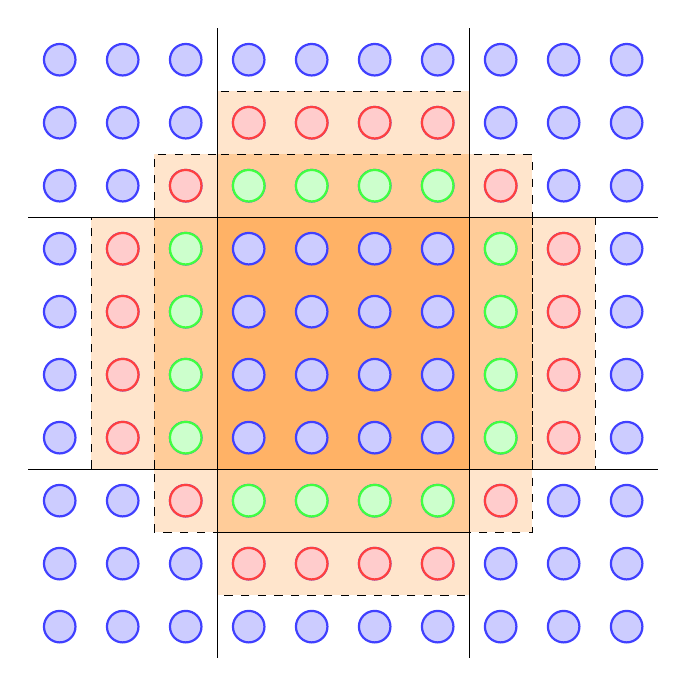
\begin{tikzpicture}[scale=0.8]
\tikzstyle{place1}=[circle,thick,draw=blue!75,fill=blue!20,minimum size=4mm]
\tikzstyle{place2}=[circle,thick,draw=green!75,fill=green!20,minimum size=4mm]
\tikzstyle{place3}=[circle,thick,draw=red!75,fill=red!20,minimum size=4mm]

\draw[dashed,fill=orange!20] (2.5,7.5) rectangle (6.5,8.5);
\draw[dashed,fill=orange!20] (2.5,0.5) rectangle (6.5,1.5);

\draw[dashed,fill=orange!20] (1.5,6.5) rectangle (0.5,2.5);
\draw[dashed,fill=orange!20] (8.5,6.5) rectangle (7.5,2.5);

\draw[dashed,fill=orange!20] (1.5,1.5) rectangle (7.5,7.5);


\draw[dashed,fill=orange!40] (2.5,6.5) rectangle (6.5,7.5);
\draw[dashed,fill=orange!40] (2.5,1.5) rectangle (6.5,2.5);

\draw[dashed,fill=orange!40] (2.5,6.5) rectangle (1.5,2.5);
\draw[dashed,fill=orange!40] (7.5,6.5) rectangle (6.5,2.5);


\draw[fill=orange!60] (2.5,2.5) rectangle (6.5,6.5);


\draw (2.5,2.5) -- (-0.5,2.5);
\draw (6.5,2.5) -- (9.5,2.5);

\draw (2.5,6.5) -- (-0.5,6.5);
\draw (6.5,6.5) -- (9.5,6.5);


\draw (2.5,2.5) -- (2.5,-0.5);
\draw (2.5,6.5) -- (2.5,9.5);

\draw (6.5,2.5) -- (6.5,-0.5);
\draw (6.5,6.5) -- (6.5,9.5);


\foreach \x in {0,...,9}
{
  \foreach \y in {0,...,9}
  {
    \node[place1] () at (\x,\y) {};
  }
}

\foreach \x in {3,...,6}
{
  \node[place2] () at (\x,2) {};
  \node[place2] () at (\x,7) {};
}
\foreach \y in {3,...,6}
{
  \node[place2] () at (2,\y) {};
  \node[place2] () at (7,\y) {};
}


\foreach \x in {3,...,6}
{
  \node[place3] () at (\x,1) {};
  \node[place3] () at (\x,8) {};
}
\foreach \y in {3,...,6}
{
  \node[place3] () at (1,\y) {};
  \node[place3] () at (8,\y) {};
}


\node[place3] () at (2,2) {};
\node[place3] () at (7,2) {};
\node[place3] () at (2,7) {};
\node[place3] () at (7,7) {};


\end{tikzpicture}
}
\end{figure}

Pour appliquer cette technique, il faut toutefois savoir à l'avance combien de fois le stencil sera itéré, cela est possible avec la syntaxe proposée pour le chaînage de stencils, mais cela n'est pas possible pour le cas général où une nouvelle syntaxe est alors nécessaire (par exemple en intercalant le nombre d'itérations dans la syntaxe présentée dans le code \ref{lst:agreg1_stencil}). 

Une nouvelles fois c'est la spécialisation partielle qui permettrait de mettre en œuvre le déclenchement automatique de l'utilisation de cette technique. C'est aussi par la spécialisation partielle que pourrait être choisie la forme la plus adaptée des blocs pour le tuilage. 


Le DSEL est cependant déjà utilisable sans toutes ces améliorations (notamment pour un problème de Jacobi), il est donc possible d'en évaluer la qualité tant au niveau du front-end que du back-end. Le chapitre suivant présente les résultats de ces évaluations concernant sommairement la qualité du front-end, et de manière plus poussée la qualité du back-end : principalement la rapidité d'exécution des problèmes.
